\documentclass[11pt]{article}

\usepackage[a4paper,margin=1in]{geometry}
\usepackage{amsmath}
\usepackage{graphicx}
\usepackage{amssymb}
\usepackage{parskip}
\usepackage[table]{xcolor}
\usepackage{tikz}
\usetikzlibrary{arrows.meta, positioning, shapes.geometric, calc}
\usepackage[most]{tcolorbox}
\usepackage{titlesec}
\usepackage{enumitem}
\usepackage{booktabs}
\usepackage{array}
\usepackage{hyperref}

% ---------- Colors ----------
\definecolor{deepblue}{HTML}{1B3B6F}
\definecolor{accent}{HTML}{2E86AB}
\definecolor{accent2}{HTML}{E07A3F}
\definecolor{soft}{HTML}{F4F7FB}
\definecolor{soft2}{HTML}{FFF4EC}
\definecolor{linegray}{HTML}{D6DEE8}
\definecolor{textgray}{HTML}{333333}
\definecolor{codebg}{HTML}{1B3B6F}
\definecolor{codefg}{HTML}{F4F7FB}

% ---------- Section styling ----------
\titleformat{\section}
  {\Large\bfseries\color{deepblue}}
  {}{0em}{}[{\color{accent}\titlerule[1.2pt]}]
\titlespacing*{\section}{0pt}{18pt}{10pt}

\titleformat{\subsection}
  {\large\bfseries\color{accent}}
  {\thesubsection}{0.6em}{}
\titlespacing*{\subsection}{0pt}{14pt}{6pt}

% ---------- Reusable boxes ----------
\newtcolorbox{codebox}{
  colback=codebg, colframe=codebg,
  coltext=codefg,
  fonttitle=\bfseries,
  boxrule=0pt, arc=3pt, outer arc=3pt,
  left=8pt, right=8pt, top=6pt, bottom=6pt,
  fontupper=\ttfamily\small
}

\newtcolorbox{stepbox}[1]{
  colback=soft, colframe=deepblue,
  boxrule=0.8pt, arc=3pt, outer arc=3pt,
  left=10pt, right=10pt, top=6pt, bottom=6pt,
  title={#1}, fonttitle=\bfseries\color{white},
  colbacktitle=deepblue, coltitle=white
}

\newtcolorbox{plainbox}{
  colback=soft, colframe=accent,
  boxrule=0.8pt, arc=3pt, outer arc=3pt,
  left=10pt, right=10pt, top=6pt, bottom=6pt
}

\newtcolorbox{warnbox}{
  colback=soft2, colframe=accent2,
  boxrule=0.8pt, arc=3pt, outer arc=3pt,
  left=10pt, right=10pt, top=6pt, bottom=6pt
}

\hypersetup{
  colorlinks=true, linkcolor=deepblue, urlcolor=deepblue
}

\begin{document}

% ---------- Title ----------
\begin{center}
  {\Huge\bfseries\color{deepblue} A Simple Tutorial on\\[2pt] On-Policy and Off-Policy Learning}\\[4pt]
  {\color{accent}\rule{0.4\linewidth}{1pt}}
\end{center}
\vspace{8pt}

\section*{What Does ``Policy'' Mean?}

A policy is simply the mechanism that decides what action or output to produce. For a language model, we write the policy as

\[
\pi_\theta(y \mid x),
\]

\begin{itemize}[leftmargin=1.4em]
  \item $x$ is the input or prompt,
  \item $y$ is a generated response,
  \item $\theta$ represents the model parameters,
  \item $\pi_\theta(y \mid x)$ is the probability that the model generates response $y$ given prompt $x$.
\end{itemize}

\begin{plainbox}
In the context of LLM training, \emph{policy} can simply be understood as \textbf{the model that generates the responses}.
\end{plainbox}

\section*{On-Policy Learning}

\subsection*{Basic Idea}

In \textbf{on-policy learning}, the training examples are generated by the \textbf{current version of the model}. Suppose the current model is $\pi_{\theta_0}$. We give it a prompt $x$ and ask it to generate several candidate responses:

\[
y_1,y_2,\ldots,y_N \sim \pi_{\theta_0}(\cdot \mid x).
\]

These responses are scored, ranked, or otherwise evaluated, and the selected responses are used to update the same model: $\pi_{\theta_0} \rightarrow \pi_{\theta_1}$.

The important point is that, in the next training round, we generate \textbf{new} responses using the \textbf{new} model $\pi_{\theta_1}$, and the process repeats.

\begin{center}
\resizebox{\textwidth}{!}{%
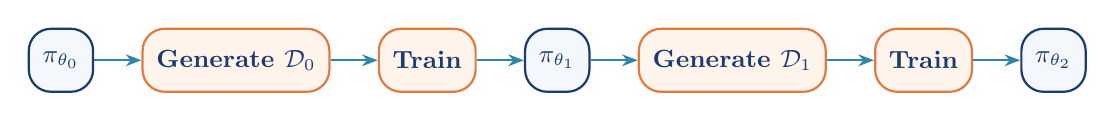
\begin{tikzpicture}[
  node distance=4mm and 6mm,
  chip/.style={rectangle, rounded corners=8pt, draw=deepblue, thick,
               fill=soft, minimum height=8mm, inner sep=5pt,
               font=\small\bfseries\color{deepblue}},
  chip2/.style={chip, fill=soft2, draw=accent2},
  arrow2/.style={-{Stealth[length=2mm]}, thick, color=accent}
]
  \node[chip] (p0) {$\pi_{\theta_0}$};
  \node[chip2, right=of p0] (g0) {Generate $\mathcal{D}_0$};
  \node[chip2, right=of g0] (t0) {Train};
  \node[chip, right=of t0] (p1) {$\pi_{\theta_1}$};
  \node[chip2, right=of p1] (g1) {Generate $\mathcal{D}_1$};
  \node[chip2, right=of g1] (t1) {Train};
  \node[chip, right=of t1] (p2) {$\pi_{\theta_2}$};

  \draw[arrow2] (p0) -- (g0);
  \draw[arrow2] (g0) -- (t0);
  \draw[arrow2] (t0) -- (p1);
  \draw[arrow2] (p1) -- (g1);
  \draw[arrow2] (g1) -- (t1);
  \draw[arrow2] (t1) -- (p2);
\end{tikzpicture}%
}
\end{center}

The generator continually follows the latest model.

\subsection*{Simple Example}

\begin{stepbox}{Prompt: What is $15 \times 4$?}
The input is the prompt $x = $ ``What is $15\times 4$?''. The current model $\pi_{\theta_t}$ generates four candidate answers:
\[
y_1 = 60,\quad y_2 = 55,\quad y_3 = 60,\quad y_4 = 45.
\]

\textbf{Where the scorer sits:} immediately after generation, before training. A scorer or evaluator (rule-based checker, reward model, or human) assigns each $(x, y_i)$ pair a score:
\[
r_1 = 1,\quad r_2 = 0,\quad r_3 = 1,\quad r_4 = 0
\]
where $r_i = 1$ denotes a correct answer (i.e.\ $y_i = 60$).

\textbf{What the training data looks like:} the stored records combine the prompt, the model's own answer, and the score:
\[
\{(x, y_1, r_1), (x, y_2, r_2), (x, y_3, r_3), (x, y_4, r_4)\}.
\]
This batch — generated by $\pi_{\theta_t}$ itself and scored immediately — is what gets used to update the model, producing $\pi_{\theta_{t+1}}$.

For the \emph{next} iteration we do not reuse these four answers — we sample fresh ones from the updated model, and the scorer evaluates \emph{those} instead:
\[
y'_1,\ldots,y'_N \sim \pi_{\theta_{t+1}}.
\]
\end{stepbox}

\begin{plainbox}
\textbf{Key idea:} on-policy means the training data is generated using the model's \textbf{current} policy.
\end{plainbox}

\subsection*{Why Does On-Policy Training Matter?}

As the model learns, the types of mistakes it makes also change. An early model may frequently produce very poor answers; after several updates those simple mistakes disappear, and the model instead makes more subtle mistakes. With on-policy training, we continuously generate new samples from the latest model:

\[
\pi_{\theta_0} \rightarrow \pi_{\theta_1} \rightarrow \pi_{\theta_2} \rightarrow \cdots
\qquad\text{and correspondingly}\qquad
\mathcal{D}_0 \rightarrow \mathcal{D}_1 \rightarrow \mathcal{D}_2 \rightarrow \cdots.
\]

This keeps the training process focused on the weaknesses of the \textbf{current} model.

\section*{Off-Policy Learning}

\subsection*{Basic Idea}

In \textbf{off-policy learning}, the responses used for training were generated by a policy \textbf{different} from the current model. For example, an older model $\pi_{\theta_0}$ or another model $\pi_B$ generates a dataset $\mathcal{D} = \{(x_i,y_i)\}_{i=1}^{M}$, which is stored and later used to train a newer model $\pi_{\theta_5}$. Since $\mathcal{D}$ was not generated by $\pi_{\theta_5}$, the training is off-policy.

\begin{center}
\resizebox{0.6\textwidth}{!}{%
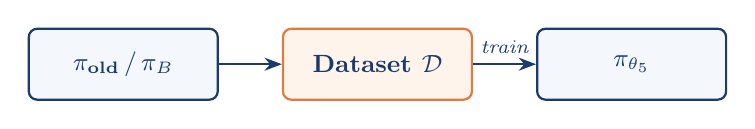
\begin{tikzpicture}[
  node distance=6mm and 8mm,
  box/.style={rectangle, rounded corners=3pt, draw=deepblue, thick,
              fill=soft, minimum width=24mm, minimum height=9mm,
              align=center, font=\small\bfseries\color{deepblue}},
  startbox/.style={box, fill=soft2, draw=accent2},
  arrow/.style={-{Stealth[length=2.2mm]}, thick, color=deepblue}
]
  \node[box] (old) {$\pi_{\text{old}} \,/\, \pi_B$};
  \node[startbox, right=of old] (data) {Dataset $\mathcal{D}$};
  \node[box, right=of data] (p5) {$\pi_{\theta_5}$};

  \draw[arrow] (old) -- (data);
  \draw[arrow] (data) -- node[above, font=\scriptsize\itshape\color{textgray}] {train} (p5);
\end{tikzpicture}%
}
\end{center}

The data-generating policy does not necessarily change together with the model being optimized.

\subsection*{Why Use Off-Policy Training?}

Generating new model outputs at every optimization step can be expensive. Off-policy learning lets us reuse previously generated data:

\[
\mathcal{D} = \{(x_i,y_i,r_i)\}_{i=1}^{M}
\]

can be generated once and reused for many gradient updates, substantially reducing generation cost. The trade-off is that the stored samples may no longer accurately represent the behavior of the current model.

\end{document}